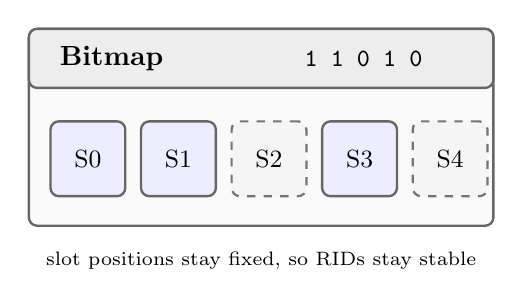
\begin{tikzpicture}[
    x=1cm,y=1cm,
    every node/.style={font=\small},
    frame/.style={draw=black!60, rounded corners=3pt, line width=0.85pt},
    slot/.style={frame, fill=blue!7, minimum width=0.95cm, minimum height=0.95cm},
    empty/.style={draw=black!55, rounded corners=3pt, line width=0.8pt, dashed, fill=gray!8, minimum width=0.95cm, minimum height=0.95cm}
]
    \draw[frame, fill=gray!4] (0,0) rectangle (5.9,2.5);
    \draw[frame, fill=gray!14] (0,1.75) rectangle (5.9,2.5);
    \node[font=\bfseries] at (1.05,2.12) {Bitmap};
    \node[font=\ttfamily\small] at (4.25,2.12) {1 1 0 1 0};

    \node[slot]  at (0.75,0.85) {S0};
    \node[slot]  at (1.90,0.85) {S1};
    \node[empty] at (3.05,0.85) {S2};
    \node[slot]  at (4.20,0.85) {S3};
    \node[empty] at (5.35,0.85) {S4};

    \node[font=\scriptsize, align=center] at (2.95,-0.45) {slot positions stay fixed, so RIDs stay stable};
\end{tikzpicture}
